
\documentclass[journal,transmag]{IEEEtran}
\hyphenation{op-tical net-works semi-conduc-tor}

\usepackage{enumitem}

\usepackage{amsmath}


% *** GRAPHICS RELATED PACKAGES ***
%
\ifCLASSINFOpdf
   \usepackage[pdftex]{graphicx}
  % declare the path(s) where your graphic files are
  % \graphicspath{{../pdf/}{../jpeg/}}
  % and their extensions so you won't have to specify these with
  % every instance of \includegraphics
  % \DeclareGraphicsExtensions{.pdf,.jpeg,.png}
\else
  % or other class option (dvipsone, dvipdf, if not using dvips). graphicx
  % will default to the driver specified in the system graphics.cfg if no
  % driver is specified.
  % \usepackage[dvips]{graphicx}
  % declare the path(s) where your graphic files are
  % \graphicspath{{../eps/}}
  % and their extensions so you won't have to specify these with
  % every instance of \includegraphics
  % \DeclareGraphicsExtensions{.eps}
\fi
% graphicx was written by David Carlisle and Sebastian Rahtz. It is
% required if you want graphics, photos, etc. graphicx.sty is already
% installed on most LaTeX systems. The latest version and documentation
% can be obtained at: 
% http://www.ctan.org/pkg/graphicx
% Another good source of documentation is "Using Imported Graphics in
% LaTeX2e" by Keith Reckdahl which can be found at:
% http://www.ctan.org/pkg/epslatex
%
% latex, and pdflatex in dvi mode, support graphics in encapsulated
% postscript (.eps) format. pdflatex in pdf mode supports graphics
% in .pdf, .jpeg, .png and .mps (metapost) formats. Users should ensure
% that all non-photo figures use a vector format (.eps, .pdf, .mps) and
% not a bitmapped formats (.jpeg, .png). The IEEE frowns on bitmapped formats
% which can result in "jaggedy"/blurry rendering of lines and letters as
% well as large increases in file sizes.
%
% You can find documentation about the pdfTeX application at:
% http://www.tug.org/applications/pdftex





\begin{document}

\title{\textsc{EXPERIMENTO 4 “ENERGY HARVESTING”-PIEZOELECTRICOS}}

\author{
\IEEEauthorblockN{Juan David Castro Bocarejo , Juan Camilo Hernandez Torres, William Andrés Gómez Roa}
\IEEEauthorblockA{Pontificia Universidad Javeriana, Bogotá, Colombia}
\IEEEauthorblockA{Laboratorio - Sistemas Dinámicos}


}
% The paper headers
\markboth{Piezoeléctrico. Mayo 02 ~2023}%
{Shell \MakeLowercase{\textit{et al.}}: Bare Demo of IEEEtran.cls for IEEE Transactions on Magnetics Journals}
\IEEEtitleabstractindextext{%

	\begin{abstract}
In this laboratory, research was conducted to understand the operation of piezoelectric elements. To achieve this objective, a rectifier circuit was implemented that allowed for observation of the signal generated by the piezoelectric element in positive values, thereby understanding how these types of devices behave. Additionally, a capacitor was used to highlight the voltage peaks generated by the element, which allowed for comparisons with other obtained values.

It is important to note that piezoelectric elements are devices that convert mechanical energy into electrical energy vice versa, making them useful in various applications such as sensors and transducers. The rectifier circuit used in this laboratory allowed for a cleaner and easier to analyze signal, as it eliminated the negative part of the signal, facilitating its analysis, and practically demonstrating the operation of these types of elements.
	\end{abstract}
	\begin{IEEEkeywords}
	Piezoelectric elements, Rectifier circuit, Electrical energy, Mechanical energy, Transducers
	 	\end{IEEEkeywords}}


\maketitle
\IEEEdisplaynontitleabstractindextext
\IEEEpeerreviewmaketitle


\section{Resumen}
En este laboratorio se llevó a cabo una investigación para comprender el funcionamiento de los elementos piezoeléctricos. Para lograr este objetivo, se implementó un circuito rectificador que permitió observar la señal generada por el piezoeléctrico en los valores positivos y de esta forma entender como se comportaba este tipo de dispositivos. Además, se utilizó un condensador para evidenciar, los picos de voltaje generados por el elemento, lo que permitió realizar comparaciones con otros valores obtenidos. 

Es importante destacar que los elementos piezoeléctricos son dispositivos que convierten la energía mecánica en energía eléctrica y viceversa, lo que los hace útiles en diversas aplicaciones, como sensores y transductores. El circuito rectificador utilizado en este laboratorio permitió obtener una señal más limpia y fácil de analizar, ya que eliminó la parte negativa de la señal, facilitando su analisis, ademas de lograr evidenciar praticamente el uncionamiento de este tipo de elementos. 
\begin{IEEEkeywords}
Elementos piezoeléctricos, Circuito rectificador, Energía eléctrica, Energía mecánica, Transductores
	 	\end{IEEEkeywords}

\section{METODOLOGÍA}

\subsection{Cálculos Previos}

\begin{enumerate}[]
  \item \textbf{Para el cristal piezoeléctrico adquirido estimar el voltaje y la energía que se puede generar al oprimirlo con los dedos.}
Ya que el cristal piezoeléctrico adquirido no cuenta con una referencia no podemos saber exactamente qué características tiene dicho PZT, pero asumiéremos valores de referencia de PIC 255 cuyo grosor es de 0.2mm y tiene un diámetro de 20mm para los cálculos.  

Además, si hacemos una fuerza con el dedo de 100N sobre este disco de área A=0.31e-3 m², entonces tendremos una Presión de 322.6 kPa.  

Utilizando un $g_33= 24.4e-3 [V-m/N] $,  tendremos un Voltaje generado de $V=1,6 Volts$. 

Finalmente, con un $d_33=400e-12 [C/N]$, tendremos una densidad de energía $u= 0.51 [nJ/mm3]$. 

  \item \textbf{De las especificaciones del diodo 1N914 suministrado ¿cuál es la máxima corriente que se puede manejar si la caída de voltaje sobre el diodo, (Forward Voltage), se debe mantener por debajo de 0,8 V?}
Observando la hoja de datos para el diodo 1N4148, el cual es homologo al 1N914, vemos por un lado que tiene un Voltaje máximo en directa de 1V. Por otro lado, observamos en la imagen que se muestra a continuación que para un Voltaje en directa de 0.8V la corriente en directa es de 10mA. 

\begin{figure}[!h]
    \center
    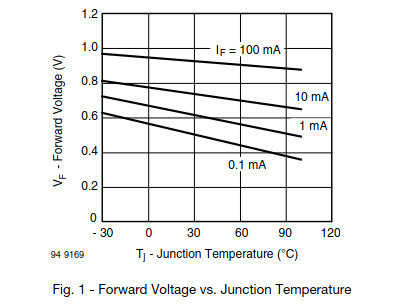
\includegraphics[width=9cm]{imgs/s1.jpeg}
    \caption{Corriente para diferentes voltajes en directa}
    \label{1}
\end{figure}

  \item \textbf{Calcular el valor del condensador necesario para el filtro si se tiene una señal de voltaje generado (voltaje de entrada) de $+- 10 V $y un periodo de 1 s. Se debe mantener la corriente en el valor especificado en b. Este condensador se debe adquirir. }

Si se desea mantener la corriente constante se debe utilizar un condensador y una resistencia a la salida del puente rectificador con el fin de mantener un voltaje constante con una corriente que fluya a través de dicha resistencia y posea una constante de tiempo  TAO.  

Si la caída sobre 1 diodo es de 0.8V, se espera que el voltaje máximo alcanzado sea de 9.2V; para este voltaje y una corriente de 10mA, tenemos una resistencia $R=920 oHm $.   Ahora si deseamos mantener un rzado algo constante para mantener la corriente constante, debemos calcular la Capacitancia para que el rizado no sea mayor que cierto valor utilizando la formula $C = I * T / Vr$, donde Vr es el voltaje de rizado. 

Si permitimos un voltaje de rizado de 1V, $I=10mA$, $T=1s$ , tenemos que $C=0.01F$.  Para adquirir el condensador seria un condensador 103. 

\item \textbf{Para un diodo LED rojo (un solo color) cual es el voltaje y la corriente requerida en el estado “ON” }

Según las hojas de datos para estos diodos LED rojos, se requiere una corriente de 16-18mA y una corriente máxima de 20mA, además la caída de voltaje sobre estos o voltaje mínimo es de 1.8-2.2 V  
\end{enumerate}

\subsection{EXPERIMENTO}
    
El procedimiento de la practica consistió en utilizar una señal sinusoidal de 1 V pico a 1 Hz del generador de señales y con la construcción de un puente rectificador de diodos 1N4148, verificar el correcto funcionamiento del rectificador de onda completa.  Además, registramos la carga y descarga de un condensador a la salida del puente rectificado a través de una resistencia en la salida del puente rectificador.  

Luego de esto utilizamos el puente rectificador para rectificar la señal que se generó al presionar un disco piezoeléctrico con el dedo y cargar un condensador con dicha señal generada. 



\section{RESULTADOS } 
A continuación, se presenta la señal de entrada generada por el DVM, medida en el osciloscopio. Ésta, como se pedía en la guía, tuvo una amplitud de 2Vpp y una frecuencia de 1 Hz. 
\begin{figure}[!h]
		\center
		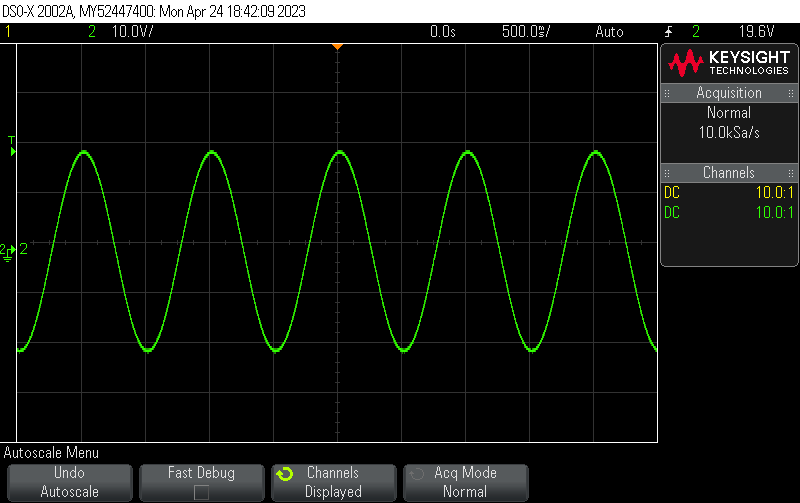
\includegraphics[width=9cm]{imgs/s2.png}
		\caption{Señal de entrada. }
		\label{1}
\end{figure}

A continuación, se muestra el resultado de la señal de entrada presentada anteriormente al ser conectada al puente de diodos, que funciona como un rectificador de onda completa. Como se observa en la imagen, el trabajo del rectificador es volver la parte negativa de la señal positiva. 

\begin{figure}[!h]
		\center
		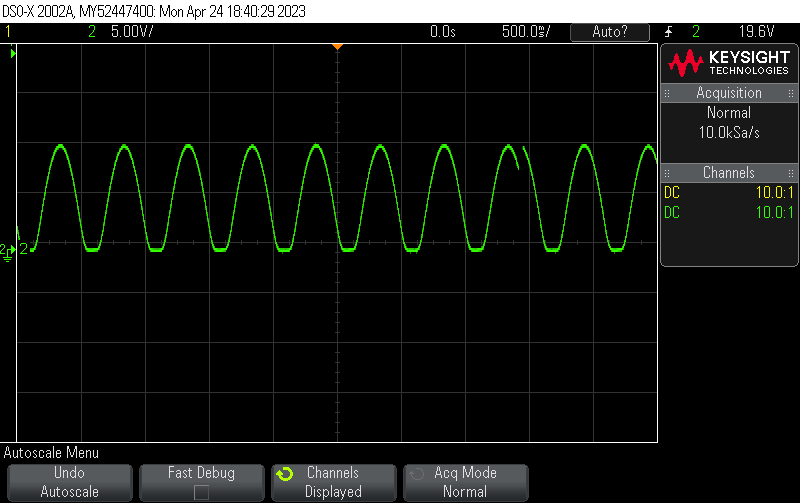
\includegraphics[width=9cm]{imgs/s3.png}
		\caption{Señal rectificada.}
		\label{2}
\end{figure}

Ahora, se presenta la misma señal de entrada del punto e. al ser expuesta al circuito del esquemático de la guía completo. En este caso, se muestran ciclos de carga y descarga del capacitor, lo que explica las bajadas suavizadas. 

\begin{figure}[!h]
    \center
    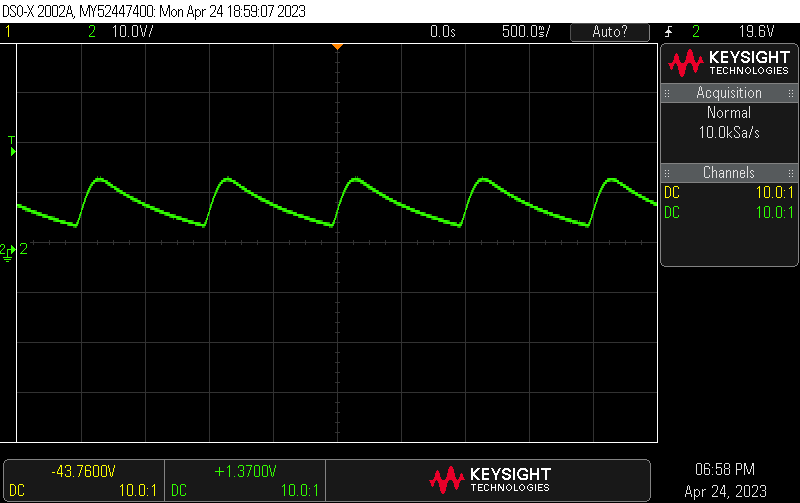
\includegraphics[width=9cm]{imgs/s4.png}
    \caption{Señal rectificada y el condensador.}
    \label{2}
\end{figure}

Señal usando el piezoeléctrico repetidas veces y dejando descargar el condensador: 

Finalmente, se muestra la Figura resultante de cargar el capacitor del circuito esquemático con el piezoeléctrico. Por ello se observa una subida de voltaje irregular, resultado de presionar repetidamente el piezoeléctrico, para finalmente soltarlo y observar la caída de voltaje, consecuencia de la descarga del condensador. 

\begin{figure}[!h]
    \center
    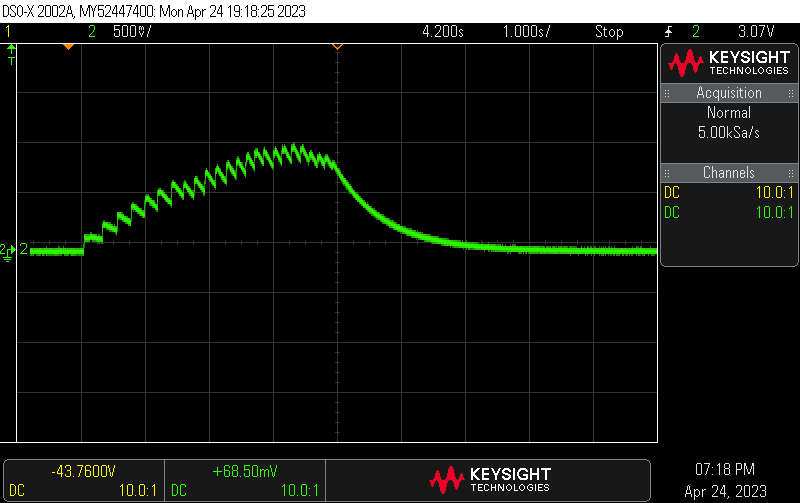
\includegraphics[width=9cm]{imgs/s5.png}
    \caption{Señal de salida piezóeléctrico.}
    \label{2}
\end{figure}
  
%%%%%%%%%%%%%%%%%%%%%%%%%%%%%%%%%%%%%%%%%%%%%%%%%%%%RESULTADOS
\section{ANÁLISIS}

En la “Figura 2. señal de entrada”, se logra observar la señal de entrada, esta es una onda sinusoidal la cual tiene un valor de pico a pico de 2v y valor pico de 1v, esta señal será rectificada por el puente de diodos, como se ve en” Figura 3. señal rectificada”, en donde se puede observar la señal de entrada rectificada ya que solo maneja valores positivos correspondientes a la señal original. Ya al agregar el condensador y medir la señal de salida, observamos el comportamiento de almacenamiento de energía del condensador, esto se evidencia en “Figura 4”, en donde se observa la señal rectificada, al condensador obteniendo su máximo valor de voltaje y como se va descargando mientras cae el voltaje, esto se realizó con el fin de probar la eficiencia del circuito y asegurarnos de su correcto funcionamiento, ya que cualquier error dentro del diseño genera que no rectifique correctamente la señal generada. 

Una vez confirmado el correcto funcionamiento de nuestro circuito, intercambiamos el generador de señales por el piezoeléctrico y comenzamos a ejercer un esfuerzo en el área del piezoeléctrico, hasta generar una deformación para generar un diferencial de voltaje, el cual medido y se observó su comportamiento en “Figura 5. señal de salida piezoeléctrico.” en la cual se observa como el valor de voltaje en el condensador depende de los picos de voltaje generados por el piezoeléctrico y como este va variando, es decir este valor cambia cada vez que se logre superar el voltaje generado por la perturbación del piezoeléctrico, la cual depende directamente del esfuerzo aplicado y de la deformación que esta sufra. 


\section{Conclusion}
	
	Inicialmente, fue posible observar la aplicación de rectificadores en la práctica. Su utilidad es evidente a la hora de utilizar corriente alterna en elementos de almacenamiento de energía con polaridad como lo son los capacitores y los LED. 

En segundo lugar, también se puso en práctica el uso de piezoeléctricos como fuentes de energía dependientes de fuerza mecánica. Es evidente que esta tecnología tiene diversas aplicaciones, pero sus reducidos tamaños y bajos voltajes previenen utilizarlos a grandes escalas. Por otro lado, esto es ideal para aplicaciones en dispositivos portátiles (wearable). 

Un ejemplo de esto lo muestran Jeong et al. [1] en un artículo en el que proponen tecnología de piezoeléctrico en la suela de los zapatos con el propósito de “cosechar energía” (energy harvesting). En general, se propone una placa piezoeléctrica unida a un resorte y ubicada a la altura del talón, como se muestra a continuación: 

\begin{figure}[!h]
    \center
    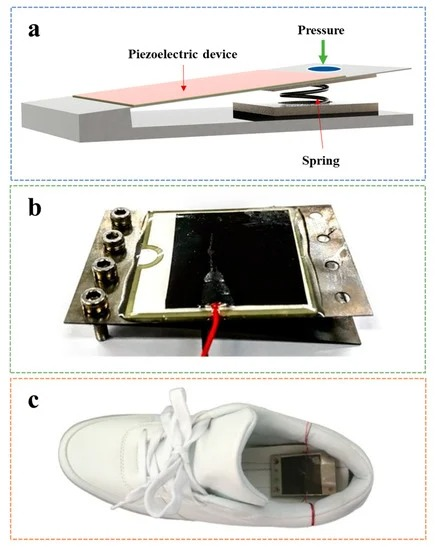
\includegraphics[width=9cm]{imgs/s6.jpeg}
    \caption{Ejemplo aplicación}
    \label{2}
\end{figure}

Esta placa está diseñada para soportar el peso sin dañar el cristal, y así mismo toma medidas para evitar daño por otros factores como la radiación UV. Posteriormente, se procede a explicar el método de almacenamiento de energía, la cual podría ser usada para cargar otros dispositivos portátiles al final de la actividad física o la caminata simple en la que se usen los zapatos. 

\appendices


\ifCLASSOPTIONcaptionsoff
  \newpage
\fi


\begin{thebibliography}{1}


 \bibitem{IEEEexample1}
   S. Y. Jeong et al., “Wearable Shoe-Mounted Piezoelectric Energy Harvester for a Self-Powered Wireless Communication System,” Energies, vol. 15, no. 1, p. 237, Dec. 2021, doi: 10.3390/en15010237. 

\end{thebibliography}


\end{document}
